\documentclass[conference]{IEEEtran}

\usepackage{newtxtext,newtxmath}
\usepackage{amsmath}
\usepackage{booktabs}
\usepackage{graphicx}
\usepackage{xcolor}
\usepackage{url}
\usepackage[hidelinks]{hyperref}
\hypersetup{
  pdftitle={QuaRM: Accounting for Data-Quality Debt Across Interacting Defects and Analytical Workloads},
  pdfauthor={AUTHOR METADATA REQUIRED BEFORE SUBMISSION},
  pdfsubject={ICDE 2027 regular research submission},
  pdfkeywords={data quality, analytical workloads, counterfactual evaluation, Shapley value}
}

\graphicspath{{../../artifacts/icde_figures/}{../../artifacts/figures/}}
% Generated by scripts/make_icde_paper_assets.py; do not edit manually.
\newcommand{\NYCRisk}{19.20}
\newcommand{\NYCDimensionDebt}{9.56}
\newcommand{\NYCDimensionLow}{8.45}
\newcommand{\NYCDimensionHigh}{10.73}
\newcommand{\MaxRelInteraction}{5.90}
\newcommand{\MLPositive}{7}
\newcommand{\MLSettings}{8}
\newcommand{\MLMaxInteraction}{2.03}
\newcommand{\SamplingTopSixtyFour}{95.8}
\newcommand{\SamplingSurfaceSixtyFour}{12.8}
\newcommand{\SamplingRMSESixtyFour}{0.206}
\newcommand{\SamplingTopOneTwentyEight}{99.0}
\newcommand{\SamplingSurfaceOneTwentyEight}{22.4}
\newcommand{\SamplingRMSEOneTwentyEight}{0.142}


\newcommand{\method}{QuaRM}
\newcommand{\players}{\mathcal{M}}
\newcommand{\coalitions}{2^{|\players|}}
\newcommand{\emptysetrisk}{R(\varnothing)}
\newcommand{\TODO}[1]{\textcolor{red}{\textbf{[#1]}}}

\title{QuaRM: Accounting for Data-Quality Debt Across\\
Interacting Defects and Analytical Workloads}

% ICDE 2027 is single-blind. Replace this block with final author metadata,
% including the ORCID of every author, before submission.
\author{\IEEEauthorblockN{\TODO{AUTHOR NAMES REQUIRED---SINGLE-BLIND SUBMISSION}}
\IEEEauthorblockA{\TODO{Affiliations, emails, and ORCIDs required before submission}}}

\begin{document}
\maketitle

\begin{abstract}
Data-quality systems count violations, detect errors, and repair cells, but these outputs do not answer a consequential question: how much does each co-occurring defect mechanism matter to the analytical workload that consumes the data? We introduce \method, a reference-based measurement system that represents data quality as a counterfactual risk surface over coalitions of defect mechanisms. A single paired execution surface supports three deliberately distinct products: Shapley accounting that exactly allocates aggregate quality debt; interaction indices that expose non-additivity; and full-context marginal gains that select an intervention for the current joint state. \method{} evaluates modest mechanism sets exactly and provides a cached permutation estimator with finite-sample control for larger sets.

We evaluate six relational defects against eight analytical SQL queries on three controlled 100K-row star schemas and a 100K-trip snapshot of official NYC taxi data, using 12 paired repetitions for all 64 coalitions. At equal 10\% prevalence, aggregate workload debt ranges from 7.19 to \NYCRisk{} risk points, pairwise interactions reach \MaxRelInteraction{} points, and query-level priorities reverse across joins, temporal rollups, counts, and averages. On NYC, dimension drift accounts for \NYCDimensionDebt{} points (95\% CI \NYCDimensionLow--\NYCDimensionHigh). Critically, the largest Shapley account is not the best current repair in all three synthetic populations and repairing it increases loss in two. In a controlled 12-mechanism study, 64 permutations recover the leading account in \SamplingTopSixtyFour\% of 400 trials while evaluating \SamplingSurfaceSixtyFour\% of 4,096 coalitions. Eight ML settings confirm that the estimand is not SQL-specific. \method{} turns ``data quality'' from an unqualified score into an auditable claim about a reference, workload, mechanism portfolio, and decision.
\end{abstract}

\begin{IEEEkeywords}
data quality, analytical workloads, counterfactual evaluation, Shapley value, data cleaning, uncertainty
\end{IEEEkeywords}

\section{Introduction}

The most convenient data-quality number is usually the least defensible. A dashboard may report 10\% missing measures, 10\% orphan keys, and 10\% duplicate facts, implicitly inviting users to compare those percentages. Yet a temporal revenue query can be insensitive to broken foreign keys and devastated by stale timestamps; a regional join can exhibit the opposite ordering. Even within one workload, defects can mask or amplify one another. Counts can absorb missing measures while duplicates inflate denominators; broken dimension links can remove precisely the tuples whose values are noisy. Prevalence is a property of the observed table. Consequence is a property of the table \emph{and its use}.

Data management has produced strong systems for detecting violations and repairing data, including constraint-based verification~\cite{schelter2018deequ}, probabilistic repair~\cite{rekatsinas2017holoclean}, and learned error detection~\cite{mahdavi2019raha}. A complementary line of work measures downstream impact: CleanML~\cite{li2021cleanml} and REIN~\cite{abdelaal2023rein} benchmark cleaning choices for machine learning (ML); JENGA~\cite{schelter2021jenga} stress-tests serving data; Foroni \emph{et al.}~\cite{foroni2021effects} derive task-specific sensitivity factors; and SAVAGE~\cite{zhu2025savage} searches for structured worst-case corruptions. These works establish that quality is task-dependent. They do not solve the accounting problem created when several declared defect mechanisms co-occur: which mechanisms account for the joint loss, which interactions defeat additive scoring, and why may the largest aggregate account differ from the best repair \emph{now}?

This distinction matters operationally. Finance may need an auditable allocation of a measured loss across upstream producers. An engineer may need the one repair that improves the current dataset most. A reliability team may need the pair of mechanisms whose interaction creates a hidden failure mode. These are different functionals of the same counterfactual response surface. Conflating them leads to a subtle but consequential error: treating an average marginal contribution over all possible contexts as if it were the marginal effect in the current context.

We introduce \method{} (Quality-Risk Measurement), illustrated in Fig.~\ref{fig:concept}. Given a trusted or explicitly provisional reference, an analytical workload and loss, and a registry of executable defect mechanisms, \method{} estimates a set function $R(S)$: the expected workload loss when exactly the mechanisms in coalition $S$ act. For a modest portfolio it evaluates all $2^m$ coalitions; for a larger portfolio it samples permutation prefixes with coalition caching. The surface yields:

\begin{itemize}
  \item an \emph{accounting estimand}: Shapley debts $\phi_i$ that uniquely satisfy efficiency, symmetry, dummy, and additivity, so $\sum_i\phi_i=R(\players)-R(\varnothing)$;
  \item a \emph{diagnostic estimand}: Shapley interaction indices $I_{ij}$ that average contextual second differences; and
  \item a \emph{decision estimand}: the full-context repair gain $g_i=R(\players)-R(\players\setminus\{i\})$ for the current joint state.
\end{itemize}

\begin{figure}[t]
  \centering
  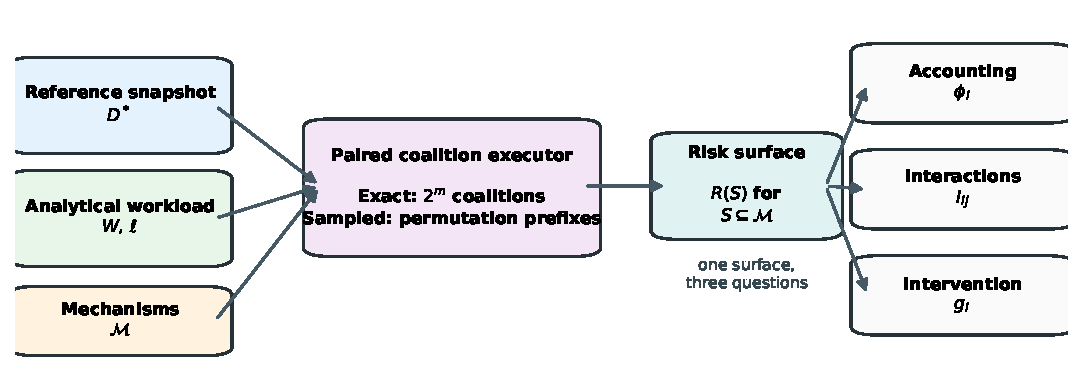
\includegraphics[width=\columnwidth]{icde_figure1_concept.pdf}
  \caption{\method{} executes a declared counterfactual contract. One risk surface supports accounting, interaction diagnosis, and current-state intervention without treating them as interchangeable.}
  \label{fig:concept}
\end{figure}

The contributions are:

\begin{enumerate}
  \item \textbf{A mechanism-coalition estimand for analytical data quality.} It applies to SQL-answer loss and predictive risk, retains signed effects, and explicitly distinguishes latent quality debt from susceptibility when the input is not verified clean.
  \item \textbf{A formal separation of accounting and intervention.} We connect exact Shapley accounting, pairwise interaction, singleton stress tests, and full-context repair within one surface, prove their relationship in additive games, and give a monotone counterexample showing that their rankings can differ.
  \item \textbf{A deterministic measurement system.} A relational backend executes eight DuckDB queries over star schemas under missing measures, value noise, orphan foreign keys, stale timestamps, dimension drift, and duplicate facts. Cryptographically derived mechanism streams make a channel invariant to coalition membership; paired bootstrap preserves this design.
  \item \textbf{Exact and sampled evaluation.} Exact enumeration provides an audit standard for modest portfolios; a cached permutation estimator is unbiased, scales as $O(Bm)$ workload evaluations before cache hits, reports standard errors, and has simultaneous Hoeffding control.
  \item \textbf{Evidence across SQL and ML.} Our checked-in study contains 2,304 generated-relational coalition repetitions, 768 NYC coalition repetitions, 1,536 ML coalition repetitions, query-level allocations, exact interactions, a 1M-row scale run, all raw observations, and SHA-256 manifests. The artifact URL is \TODO{public repository/DOI required}.
\end{enumerate}

The claim is intentionally bounded. \method{} is not an error detector, a repair generator, or a universal grade. It is a measurement layer that turns detector outputs or hypothesized failure modes into consequences under a declared workload. This boundary is what makes the resulting number scientifically interpretable.

\section{Related Work}

\subsection{Quality dimensions, detection, and repair}

Data consumers have long described quality as multidimensional and contextual~\cite{wang1996beyond}. Modern systems operationalize parts of this view. Deequ computes scalable analyzers and verifies constraints~\cite{schelter2018deequ}; Raha combines detector signals with limited labels~\cite{mahdavi2019raha}; HoloClean integrates constraints, statistics, and external information for probabilistic repair~\cite{rekatsinas2017holoclean}. Recent mixed-error systems coordinate or learn repairs: Lopster moves dirty records toward a learned clean region~\cite{reis2024lopster}, while UniClean unifies cleaners and optimizes their workflow~\cite{ding2025uniclean}. These systems produce violations or repaired values. \method{} consumes a mechanism and measures its workload consequence; it neither competes on cell-level detection F1 nor assumes that repair accuracy equals analytical utility.

\subsection{Downstream impact and stress testing}

CleanML systematically evaluates error types, cleaners, datasets, and classification models~\cite{li2021cleanml}; REIN broadens the benchmark to 38 detection and repair methods, 14 datasets, and several ML tasks~\cite{abdelaal2023rein}. JENGA injects production-inspired errors into serving data and tests whether validation schemas catch consequential failures~\cite{schelter2021jenga}. Foroni \emph{et al.} make perhaps the closest conceptual observation: quality should include a task-conditioned sensitivity factor estimated through systematic noise generation~\cite{foroni2021effects}. SAVAGE advances stress testing by searching causally inspired dependency graphs for plausible, high-impact corruption patterns~\cite{zhu2025savage}.

\method{} differs in objective and mathematical object. Prior benchmarks compare dirty, clean, or repaired variants, and stress testers measure or maximize the impact of selected corruptions. \method{} estimates the complete coalition response surface for a declared mechanism portfolio. This enables exact joint-loss accounting, interaction indices, and current-state intervention from the same executions. It supports relational SQL workloads in addition to ML and never describes its random mechanisms as worst-case or realistic by construction. SAVAGE and \method{} are complementary: a structured corruption discovered by SAVAGE can become a \method{} player; \method{} then quantifies how that player shares joint debt and interacts with other operational failure modes.

\subsection{Data valuation and cooperative games}

Data Shapley assigns predictive utility to training records~\cite{ghorbani2019datashapley}; Data Banzhaf targets robustness to noisy utility~\cite{wang2023banzhaf}; OpenDataVal demonstrates that valuation methods behave differently across downstream selection tasks~\cite{jiang2023opendataval}. \method{} uses cooperative-game machinery but is not record valuation. Its few players are executable \emph{defect mechanisms}, its value is a bounded workload loss, and its efficiency identity is an accounting control. We use the Shapley interaction index~\cite{grabisch1999interaction} to diagnose non-additivity. Most importantly, we do not infer that the largest Shapley value is the best repair. The former averages a marginal across every predecessor context; the latter is one marginal at the fully defective context.

\section{Counterfactual Quality as a Risk Surface}

\subsection{Experimental contract}

Let $D^*$ be a reference database or training sample and $W=\{q_1,\ldots,q_k\}$ an analytical workload. Each $q$ maps a database to an answer vector; an ML training-and-evaluation pipeline is also a query in this broad sense. Let $\ell_q\in[0,1]$ compare the answer under intervention with a reference answer. Let $\players=\{1,\ldots,m\}$ index named stochastic defect mechanisms. Mechanism $i$ is an operator $C_i(\theta_i,\xi_i)$ with declared severity $\theta_i$ and randomness $\xi_i$. A fixed priority order defines composition $C_S$ for $S\subseteq\players$.

The coalition risk is
\begin{equation}
 R(S)=\mathbb{E}_{\omega,\xi}\left[\sum_{q\in W}\alpha_q
 \ell_q\!\left(q(C_S(D^*;\xi)),q(D^*)\right)\right],
 \label{eq:risk}
\end{equation}
where $\alpha_q\ge 0$, $\sum_q\alpha_q=1$, and $\omega$ represents population sampling, query, split, or learner randomness. For SQL, we use bounded normalized $L_1$ answer distance and equal query weights. For ML, $q$ trains on $C_S(D^*)$ and $\ell_q$ is clean-test error. The \emph{quality debt} of $S$ is $Q(S)=R(S)-R(\varnothing)$; aggregate debt is $Q(\players)$. Negative debt is allowed: a nominal corruption can regularize a misspecified learner or attenuate another defect. Suppressing its sign would falsify the estimand.

Equation~\ref{eq:risk} is a contract, not an intrinsic dataset property. Change the workload, reference, mechanism implementation, severity, composition order, or population and the estimand changes. This is a feature: every reported number states what it is a number \emph{of}.

\subsection{Exact accounting}

For mechanism $i$, the Shapley debt is
\begin{equation}
 \phi_i=\sum_{S\subseteq\players\setminus\{i\}}
 \frac{|S|!(m-|S|-1)!}{m!}\big[R(S\cup\{i\})-R(S)\big].
 \label{eq:shapley}
\end{equation}
It is the marginal risk of adding $i$, averaged uniformly over positions in all mechanism orders. By Shapley's characterization~\cite{shapley1953value}, it is the unique allocation satisfying efficiency, symmetry, dummy, and additivity. In particular,
\begin{equation}
 \sum_{i\in\players}\phi_i=R(\players)-R(\varnothing).
 \label{eq:efficiency}
\end{equation}
We retain the signed residual of Eq.~\ref{eq:efficiency} as an implementation invariant. It is zero to floating-point precision in every reported exact study. The normalized Banzhaf value is a useful valuation comparator, but it is not efficient in general; its residual is therefore reported rather than silently renormalized.

\subsection{Interactions}

A one-defect-at-a-time study sees $R(\{i\})-R(\varnothing)$. It misses the discrete second difference
\begin{equation}
 \Delta_{ij}(S)=R(S\cup\{i,j\})-R(S\cup\{i\})-R(S\cup\{j\})+R(S).
\end{equation}
\method{} reports the Shapley interaction index $I_{ij}$, the factorially weighted average of $\Delta_{ij}(S)$ over backgrounds $S\subseteq\players\setminus\{i,j\}$~\cite{grabisch1999interaction}. Positive values indicate super-additive harm; negative values indicate attenuation. An interaction is about the executable mechanisms and workload, not a universal causal relation between abstract dimensions such as completeness and consistency.

\subsection{Accounting is not intervention}

If all mechanisms are currently present, removing $i$ yields the full-context gain
\begin{equation}
 g_i=R(\players)-R(\players\setminus\{i\}).
 \label{eq:gain}
\end{equation}
Thus $\phi_i$ answers ``how much joint debt should $i$ account for across all contexts?'' while $g_i$ answers ``what happens if we remove $i$ from this context?'' The singleton effect $s_i=R(\{i\})-R(\varnothing)$ answers a third question.

\textbf{Proposition 1 (agreement under additivity).} If $R(S)=R(\varnothing)+\sum_{i\in S}w_i$, then $s_i=\phi_i=g_i=w_i$ for every $i$. A disagreement between any of these quantities certifies non-additivity.

\emph{Proof.} Every marginal $R(S\cup\{i\})-R(S)$ equals $w_i$, so both the Shapley average and the two endpoint marginals equal $w_i$. \hfill$\square$

The converse ranking claim is false even for a monotone bounded surface. For mechanisms $A,B,C$, let
\begin{align*}
&R(\varnothing)=0,\quad R(A)=.4,\ R(B)=R(C)=.1,\\
&R(AB)=.6,\ R(AC)=.4,\ R(BC)=.5,\ R(ABC)=.8.
\end{align*}
Then $\phi=(.367,.267,.167)$, so accounting ranks $A$ first, but $g=(.3,.4,.2)$, so intervention ranks $B$ first. No estimator error is involved; the objectives differ.

\subsection{Reference boundary}

If $D^*$ is verified, $Q$ estimates debt relative to that reference. If the only available table is an observed, potentially dirty $D$, adding synthetic defects measures \emph{susceptibility}: the incremental response around $D$. Latent observed debt is not identifiable without assumptions because the same $D$ can arise from different clean references and corruption processes with different $R(\varnothing)$. Our NYC experiment is therefore labeled a real-snapshot susceptibility study, not an assertion that TLC records are clean. A curated gold subset, prior validated snapshot, simulator, or domain adjudication can strengthen the reference claim.

\section{System and Estimation}

\subsection{Relational execution}

The relational backend materializes a star schema in DuckDB~\cite{raasveldt2020duckdb}: customer and product dimensions plus an order fact table. Its eight queries cover average order value by segment, customers by region, daily revenue, orders by status, refund rate by region, revenue by category, monthly revenue, and revenue by region. These templates deliberately span aggregates, joins, grouping, filters, and temporal bucketing.

For an answer vector $a$ and clean answer $a^*$, columns are aligned on group keys; absent groups receive zero. The query loss is
\begin{equation}
 \ell_q(a,a^*)=\min\!\left\{1,
 \frac{\|a-a^*\|_1}{\|a^*\|_1+\epsilon}\right\}.
\end{equation}
The workload risk is the mean over queries. Boundedness makes risks comparable, limits domination by monetary scale, and supports distribution-free concentration. Per-query values remain available; the average does not erase the workload profile.

\subsection{Mechanism semantics}

At severity $\theta$, the relational registry implements:

\begin{itemize}
  \item \emph{missing measures}: null monetary fact values;
  \item \emph{value noise}: multiplicative perturbation of monetary measures;
  \item \emph{orphan foreign keys}: replace selected keys with absent identifiers;
  \item \emph{stale timestamps}: shift selected event times backward;
  \item \emph{dimension drift}: alter selected dimensional labels; and
  \item \emph{duplicate facts}: append selected fact rows.
\end{itemize}

Each operator has a fixed priority because composition can matter. Within repeat $r$, mechanism $i$ receives a pseudorandom stream derived by SHA-256 from the master seed, $r$, and its name. Consequently, the rows and perturbations selected by $i$ are identical whether evaluated alone or beside another mechanism. Every coalition in the repeat uses the same reference draw. This \emph{subset-invariant paired design} prevents a marginal comparison from substituting a different corruption realization.

The ML backend follows the same contract with missing cells, numeric feature noise, target noise, and duplicate rows. It evaluates logistic/ridge and random-forest pipelines from scikit-learn~\cite{pedregosa2011sklearn} on clean held-out data. The purpose is generality, not a claim that these four random mechanisms exhaust real ML failures.

\subsection{Exact evaluator and paired uncertainty}

For $m$ mechanisms and $n$ repeats, exact evaluation performs $n2^m$ workload executions. Within a repeat, it computes the reference answers once, applies every coalition, records realized mechanism diagnostics, and stores the total and per-query losses. Exact Shapley values and interactions are functions of the $2^m$ coalition means.

Uncertainty is estimated by bootstrapping complete repeats~\cite{efron1993bootstrap}. A bootstrap draw resamples the same repeat indices for every coalition, recomputes all means, and then recomputes the exact allocation. Resampling coalition rows independently would destroy the pairing. We report percentile intervals, $\Pr(\phi_i>0)$, and rank-one frequency as design-based uncertainty summaries. They are not posterior probabilities about intrinsic data quality.

Pairing also changes estimator variance. For a marginal $L_{S\cup i}-L_S$ over $n$ repeats,
\begin{equation}
 \mathrm{Var}(\widehat\Delta)=\frac{\mathrm{Var}(L_{S\cup i})+\mathrm{Var}(L_S)-2\mathrm{Cov}(L_{S\cup i},L_S)}{n}.
\end{equation}
Pairing is beneficial when within-repeat covariance is positive, not by fiat. The artifact preserves raw repetitions so this assumption can be inspected.

\subsection{Permutation estimator}

Exact enumeration is appropriate for a small operational vocabulary, but not for dozens of mechanisms. A uniformly random permutation $\pi$ supplies one marginal sample per player: if $P_i^\pi$ precedes $i$, then $X_i^\pi=R(P_i^\pi\cup\{i\})-R(P_i^\pi)$. For $B$ independent permutations,
\begin{equation}
 \widehat\phi_i=\frac{1}{B}\sum_{b=1}^B X_i^{\pi_b}.
\end{equation}

\textbf{Proposition 2 (unbiasedness and fixed-budget control).} $\mathbb{E}[\widehat\phi_i]=\phi_i$. If $R\in[0,1]$, then with probability at least $1-\delta$, simultaneously for all $m$ mechanisms,
\begin{equation}
 |\widehat\phi_i-\phi_i|\le
 \sqrt{\frac{2\log(2m/\delta)}{B}}.
 \label{eq:hoeffding}
\end{equation}

\emph{Proof sketch.} Every subset appears as $i$'s predecessor with exactly the factorial weight in Eq.~\ref{eq:shapley}, proving unbiasedness~\cite{castro2009sampling}. Each marginal lies in $[-1,1]$; Hoeffding's inequality for an interval of length two and a union bound over $m$ players give Eq.~\ref{eq:hoeffding}. \hfill$\square$

The executor caches every visited prefix coalition. Without cache hits, a permutation needs $m+1$ risks and the estimator costs $O(Bm)$ instead of $O(2^m)$. The cache also makes the actual evaluated fraction observable. Standard errors are computed from the $B$ marginal samples. The bound is conservative; empirical convergence determines practical budgets.

\subsection{Reproducibility contract}

The implementation separates mechanism definitions, coalition evaluation, attribution, sampling, relational data loading, and serialization. It emits raw coalition observations, query-specific losses, allocations, interactions, manifests, file hashes, runtime, dependency versions, and figures. Public NYC inputs are downloaded only from the official TLC endpoint and verified against pinned SHA-256 hashes. Twenty-three tests cover coalition completeness, efficiency, exact corruption counts, non-mutation, subset-invariant streams, deterministic replay, DuckDB execution, NYC loading, Banzhaf non-efficiency, sampling convergence, and the controlled 12-player surface.

\section{Experimental Method}

\subsection{Research questions}

We ask:

\begin{itemize}
  \item \textbf{RQ1: Workload context.} Does equal defect prevalence yield different debts across relational populations and SQL queries?
  \item \textbf{RQ2: Joint accounting.} Are interactions material, and does exact Shapley accounting close the aggregate debt where Banzhaf does not?
  \item \textbf{RQ3: Decision distinction.} Do Shapley accounting, singleton stress, and full-context repair select the same mechanism?
  \item \textbf{RQ4: Cost.} How do exact runtime and sampled accuracy scale?
  \item \textbf{RQ5: Generality.} Do signed, setting-dependent debts also appear in ML pipelines?
\end{itemize}

\subsection{Relational references and workload}

Three deterministic generators create 100,000-fact retail schemas. \emph{Uniform} distributes dimension membership and events evenly. \emph{Skewed} introduces long-tailed entities and categories. \emph{Seasonal} concentrates timestamps and values in time. The fourth reference is a deterministic 100,000-row sample of January 2025 NYC TLC Yellow Taxi trips~\cite{nyctlc2025}. Pickup locations form the geographic dimension, payment type forms a second dimension, and trips form facts. We filter structurally invalid timestamps and amounts before sampling but make no latent cleanliness claim.

All six mechanisms have 10\% nominal prevalence. We evaluate all 64 coalitions for 12 paired repeats and all eight queries, then perform 2,000 repeat-level bootstrap draws. Thus each population contains 768 coalition repetitions and 6,144 query executions. The TLC study uses the same frozen protocol after its hashes and loader were fixed.

\subsection{Comparators and metrics}

Equal prevalence is the non-contextual baseline; uniform repair is its implied expected one-step decision. The singleton score $s_i$ represents one-mechanism-at-a-time stress testing. Normalized Banzhaf values provide a non-efficient allocation comparator. Exact Shapley provides the proposed accounting estimand, and $g_i$ is the retrospective full-context repair oracle for the stated one-step objective. We report bounded risk points (100 times loss), bootstrap intervals, maximum absolute interaction, allocation residual, realized repair gain, and oracle regret.

For sampling, a controlled 12-mechanism surface contains unequal main effects, eight pair interactions, and three triple interactions passed through a logistic link, making all 4,096 risks bounded. Exact Shapley is ground truth. For each $B\in\{4,8,16,32,64,128,256,512\}$ we run 400 seeds and report RMSE, rank-one recovery, and unique coalition fraction.

The scale study evaluates one exact six-mechanism repeat (64 coalitions, 512 SQL query executions) at 10K, 100K, and 1M facts on the same machine. It measures end-to-end Python intervention, DuckDB loading, query execution, and loss computation; it is not a pure database microbenchmark.

\subsection{ML confirmation}

The confirmatory study covers Breast Cancer and Wine classification, Diabetes regression, and a pinned nonlinear synthetic classification population. Each uses a linear and forest model, four defect mechanisms at 15\%, 16 exact coalitions, 12 paired train/test repeats, and 2,000 bootstrap draws. Classification uses error rate; regression uses clipped IQR-normalized absolute error. It is intentionally smaller than CleanML or REIN: the question is whether the surface estimand transfers, not whether \method{} is a superior cleaner.

\subsection{Evaluation discipline}

The units of repetition are corruption/population seeds or ML splits, not datasets sampled from a hypothetical population of all applications. We therefore avoid a significance test across four references or eight ML settings. Intervals quantify repeated-protocol uncertainty within a declared setting. The exact and sampled studies use different goals: the former validates substantive relational findings; the latter isolates estimator error against known ground truth. Every number in the paper is generated from checked-in CSV evidence rather than hand-entered into the manuscript.

\section{Results}

\subsection{RQ1: Consequence depends on population and query}

Table~\ref{tab:relational} summarizes the relational surfaces. Aggregate quality debt is 7.19, 8.84, and 7.23 risk points in the three generated populations, but \NYCRisk{} points on NYC. Equal prevalence therefore does not imply equal joint consequence. Exact efficiency residual is zero in all four; all displayed total debt is allocated.

% Generated by scripts/make_icde_paper_assets.py; do not edit manually.
\begin{table*}[t]
\caption{Relational results at 10\% prevalence. Risk, allocations, and gains are percentage points of bounded workload-answer loss. $\phi$ is the top Shapley account; $g^*$ is the best full-context repair. Negative $g(\arg\max\phi)$ means that repairing the largest aggregate account alone worsens the current joint state.}
\label{tab:relational}
\centering\small\setlength{\tabcolsep}{4.3pt}
\begin{tabular}{lrrrrlllrr}
\toprule
Reference & rows & $R(\mathcal{M})$ & $Q(\mathcal{M})$ & $\max|I_{ij}|$ & top $\phi$ & Shapley repair & best repair & $g(\arg\max\phi)$ & $g^*$ \\
\midrule
NYC Taxi & 100{,}000 & 19.20 & 19.20 & 5.62 & dimension drift & dimension drift & dimension drift & 8.11 & 8.11 \\
Uniform & 100{,}000 & 7.19 & 7.19 & 5.87 & duplicate facts & duplicate facts & stale time & -0.24 & 1.52 \\
Skewed & 100{,}000 & 8.84 & 8.84 & 5.69 & duplicate facts & duplicate facts & dimension drift & 0.20 & 1.65 \\
Seasonal & 100{,}000 & 7.23 & 7.23 & 5.90 & duplicate facts & duplicate facts & stale time & -0.28 & 1.58 \\
\bottomrule
\end{tabular}
\end{table*}


Figure~\ref{fig:attributions} shows that even the aggregate mechanism profile changes. Duplicate facts lead the generated populations at approximately 2.3 points, while dimension drift dominates NYC at \NYCDimensionDebt{} points (95\% CI \NYCDimensionLow--\NYCDimensionHigh; rank-one frequency 1.0). The difference is interpretable rather than cosmetic: NYC regional and refund queries depend strongly on geographic dimension membership, while the generated reference spreads more workload mass across count, value, and temporal queries.

\begin{figure*}[t]
  \centering
  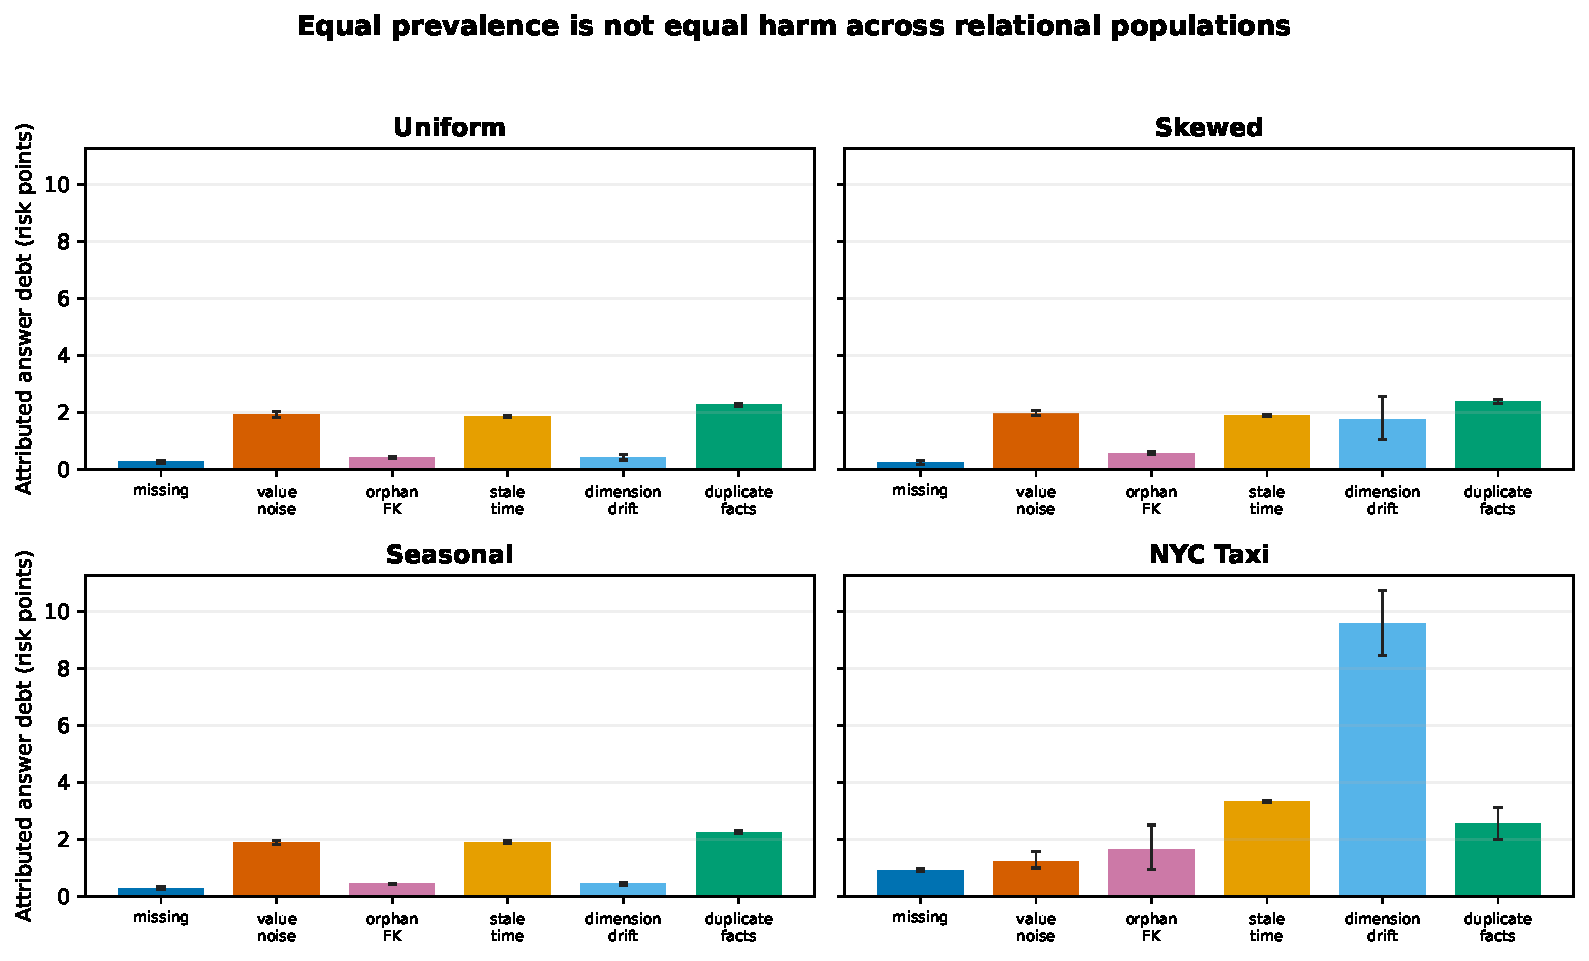
\includegraphics[width=0.97\textwidth]{icde_figure2_all_relational_attributions.pdf}
  \caption{Exact Shapley debt at equal 10\% mechanism prevalence. Bars are point allocations; whiskers are paired 95\% bootstrap intervals over 12 complete surface repetitions. The real snapshot changes the dominant account.}
  \label{fig:attributions}
\end{figure*}

The workload average hides purposeful heterogeneity. Across the 24 generated population/query combinations, the leading account is dimension drift for seven, stale timestamps for six, duplicate facts for six, value noise for three, and missing measures and orphan keys for one each. On NYC, value noise leads average-order-value, stale timestamps lead both time rollups, duplicate facts lead status/category summaries, and dimension drift leads all region-sensitive joins. This is the central failure of a dataset-only grade: no single ordering survives a change of query.

Figure~\ref{fig:queries} resolves this variation below the workload mean. Mechanisms also change sign by query. For example, dimension drift is strongly harmful to revenue-by-region in the Skewed population but slightly beneficial to some other aggregates because reassigned dimension members redistribute denominators and group support. A dashboard that stores one ``dimension accuracy'' weight would have to average away precisely the query structure needed to explain the result. Per-query surfaces avoid this collapse; the workload surface is then a declared weighted aggregation, not an irreversible score.

\begin{figure*}[t]
  \centering
  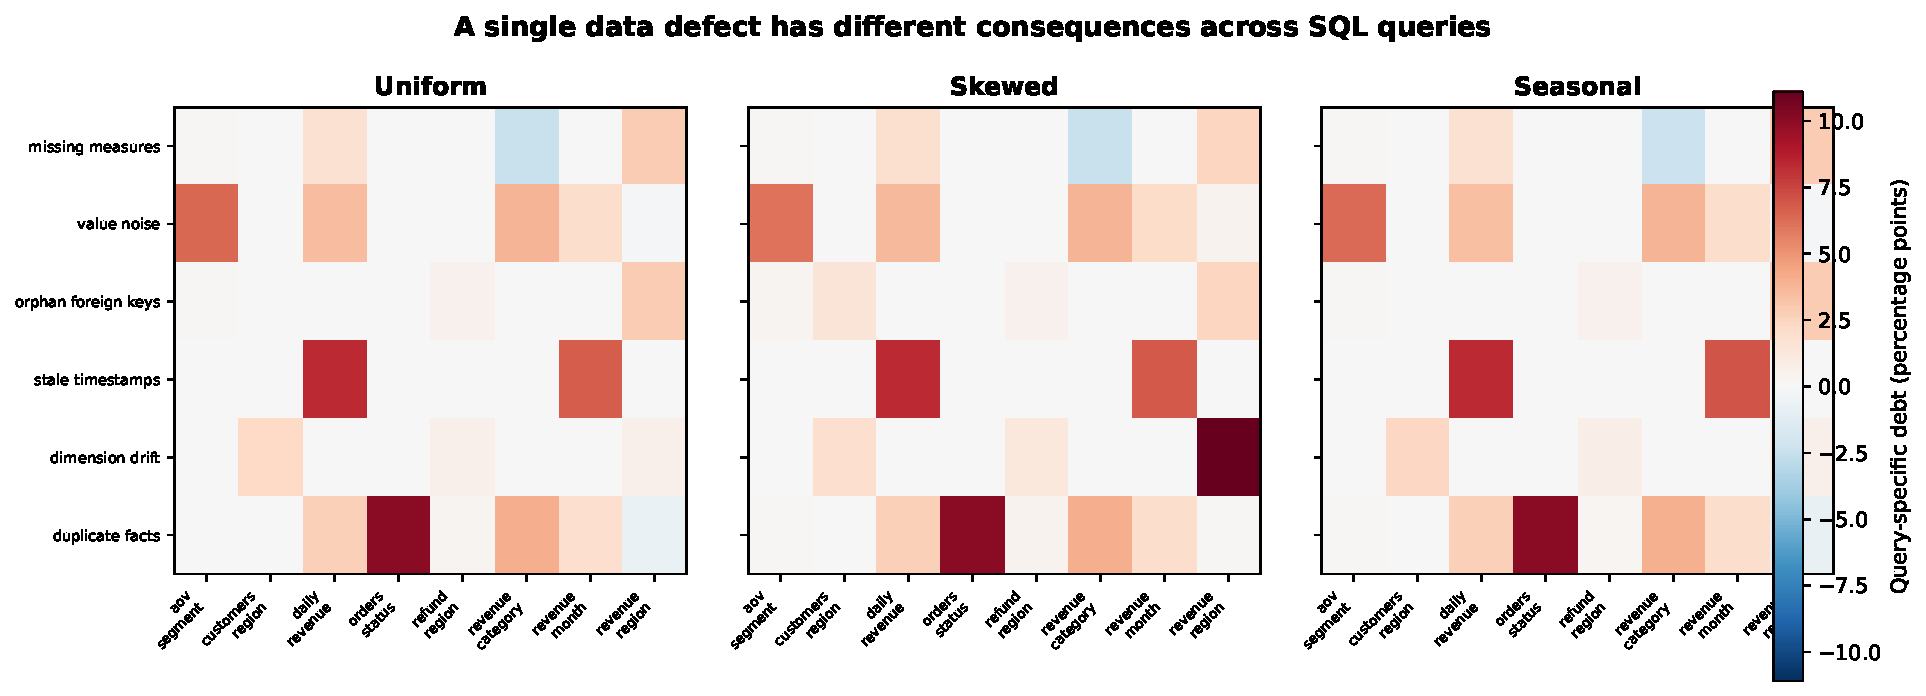
\includegraphics[width=0.96\textwidth]{icde_figure3_query_profiles.pdf}
  \caption{Query-specific Shapley allocations for the three generated populations. Red is harmful, blue is beneficial, and near-white is inert. The same 10\% mechanism can dominate one query and vanish or change sign in another.}
  \label{fig:queries}
\end{figure*}

\subsection{RQ2: Interactions are first-order evidence}

Maximum absolute interactions range from 5.62 to \MaxRelInteraction{} risk points---large relative to total generated debt. In every population the strongest interaction is negative between missing measures and duplicate facts (NYC: $-5.62$ points; generated: approximately $-5.7$ to $-5.9$). Duplication repeats rows whose measures may be null, while normalized aggregates and SQL null semantics prevent their harms from adding independently. NYC also exhibits $-3.53$ points between missing measures and value noise and $+1.90$ points between missingness and timestamp staleness.

These magnitudes explain why isolated sensitivities cannot be summed. Banzhaf allocations miss aggregate debt by $-1.89$ points on NYC and $-1.40$ to $-1.56$ points on the generated references. That is not a defect of Banzhaf for its robustness objective; it is evidence that allocation choice must match the required invariant. When the requirement is ``account for this measured total,'' efficiency is non-negotiable.

Pairing is also not an unconditional precision trick. In a design ablation that independently resamples the 12 repetitions of each coalition, the median paired-to-independent 95\% interval-width ratio is 1.20 on NYC, 1.37 on Uniform, 1.65 on Seasonal, but only 0.31 on Skewed; individual mechanism ratios range from 0.10 to 3.66. Shared repeat difficulty can induce positive covariance and narrow a marginal, while competing mechanisms can induce negative covariance and widen it. We retain pairing because it identifies like-for-like counterfactual differences and prevents intervention drift, not because it always produces a smaller interval.

\subsection{RQ3: The largest account need not be the best repair}

Figure~\ref{fig:decision} juxtaposes $\phi_i$ with $g_i$ from the same exact surface. On NYC, both objectives select dimension drift and its removal reduces workload loss by 8.11 points. On all three generated populations, however, duplicate facts have the largest aggregate Shapley account but a different mechanism has the largest current marginal: stale timestamps for Uniform and Seasonal, dimension drift for Skewed.

\begin{figure*}[t]
  \centering
  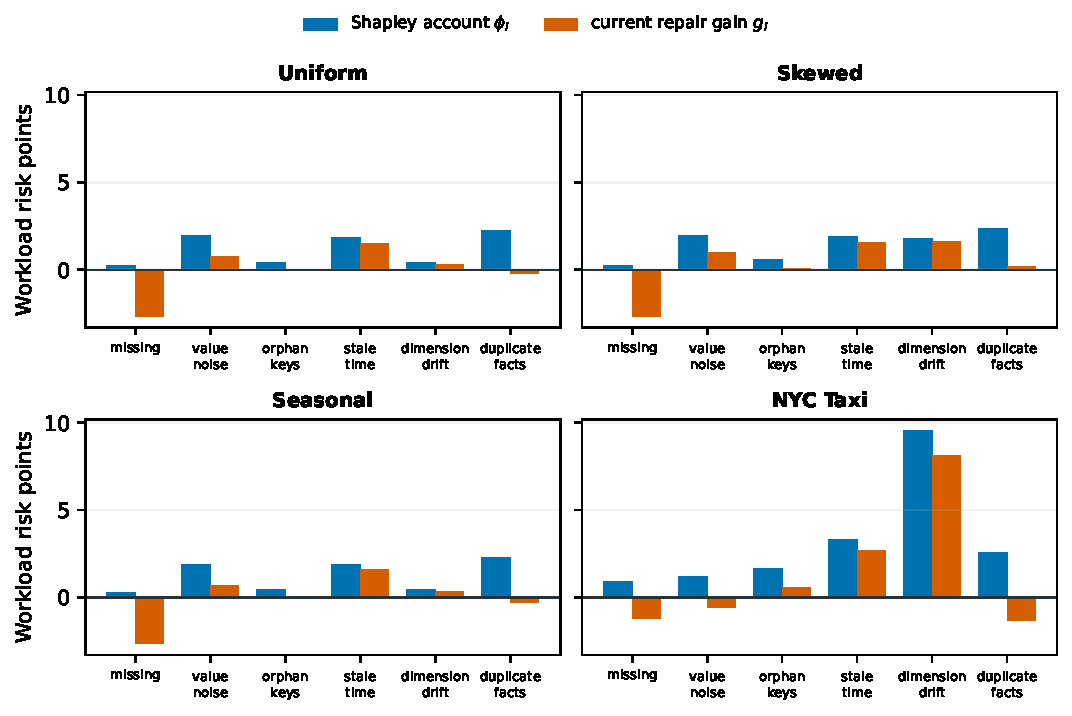
\includegraphics[width=0.95\textwidth]{icde_figure4_accounting_decision.pdf}
  \caption{Accounting versus intervention. Blue bars average each mechanism's marginal over every context; orange bars measure removal from the fully defective context. Negative orange bars are not contradictions: attenuation can make a standalone removal harmful unless another mechanism is repaired too.}
  \label{fig:decision}
\end{figure*}

The decision error is not merely a near-tie. Removing the top Shapley account \emph{increases} current loss by 0.24 points on Uniform and 0.28 on Seasonal, whereas the best repairs reduce it by 1.52 and 1.58. On Skewed, Shapley-first gains 0.20 versus the oracle's 1.65. The singleton choice equals the Shapley choice in these regimes and therefore has the same regret. Equal-prevalence uniform repair yields only the mean current marginal.

This result changes how attributions should be deployed. $\phi$ is appropriate for reporting responsibility across possible co-occurrence/repair orders. $g$ is appropriate for a one-step action given the current joint state and a perfect mechanism removal. For sequential cleaning with costs, neither alone is sufficient; one must optimize a path or policy on the surface. Calling Shapley a repair heuristic would weaken an otherwise exact accounting guarantee.

\subsection{RQ4: Exact execution and sampled scaling}

One exact six-mechanism repetition takes 9.55~s at 10K facts, 22.17~s at 100K, and 97.22~s at 1M. The 1M run includes 64 materializations and 512 analytical query executions. Runtime grows sublinearly from 10K to 100K and about $4.4\times$ from 100K to 1M, with fixed orchestration overhead visible at small scale. Repeats and coalitions are embarrassingly parallel, although the reference implementation executes them serially for deterministic resource use.

For larger $m$, Fig.~\ref{fig:sampling} shows the cost-accuracy frontier. At $m=12$, 64 permutations have median RMSE \SamplingRMSESixtyFour{} risk points, recover the exact top account in \SamplingTopSixtyFour\% of 400 trials, and evaluate \SamplingSurfaceSixtyFour\% of the surface. At 128, these become \SamplingRMSEOneTwentyEight{}, \SamplingTopOneTwentyEight\%, and \SamplingSurfaceOneTwentyEight\%. The cache fraction is crucial: ``$Bm$ evaluations'' overstates actual work when permutation prefixes repeat, but a six-player study understates scalability because its 64-coalition surface saturates. The 12-player design avoids that artifact.

\begin{figure}[t]
  \centering
  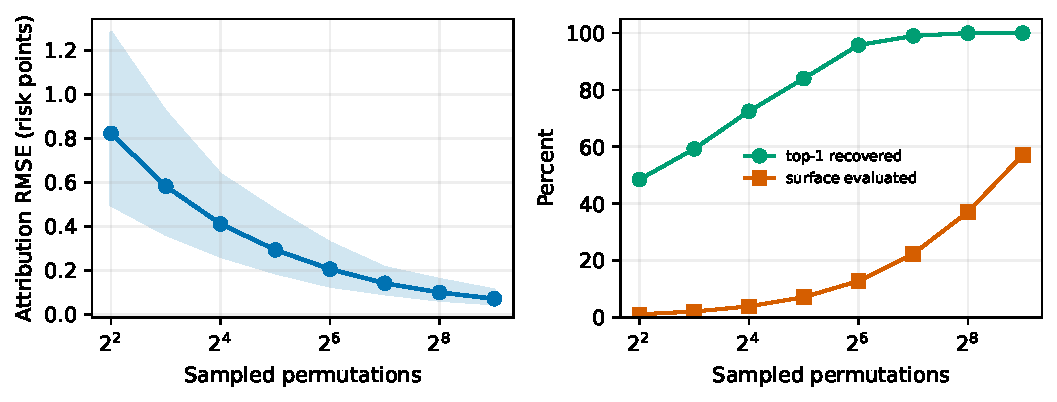
\includegraphics[width=\columnwidth]{icde_figure4_sampling_m12.pdf}
  \caption{Permutation approximation on a bounded non-additive 12-mechanism surface (400 trials per budget). Shading is the 10th--90th RMSE percentile.}
  \label{fig:sampling}
\end{figure}

The Hoeffding radius in Eq.~\ref{eq:hoeffding} is intentionally conservative and should not be mistaken for an empirical error bar. The reported standard errors and convergence plot support budget selection; the bound supplies worst-case fixed-budget coverage when its assumptions are acceptable.

The actual six-mechanism relational surfaces expose the other side of this tradeoff. With 64 permutations, median RMSE is similarly 0.205 risk points, but top-one recovery is 72.3\% and the cache has already touched 98.2\% of the 64 coalitions; at 128 it recovers 84.8\% after essentially exhausting the surface. The lower rank recovery reflects the small gap between leading mechanisms in Skewed, not large numeric error. Exact evaluation is therefore the correct default when $m=6$; sampling is a scaling strategy for larger portfolios, not a reason to approximate a small auditable game.

\subsection{RQ5: The estimand transfers to ML}

Aggregate debt is positive in \MLPositive{} of \MLSettings{} ML settings. At identical 15\% prevalence, target noise leads three settings, feature noise three, missing cells two, and random duplicates none. Pairwise interactions reach \MLMaxInteraction{} risk points. The remaining setting---a linear learner on nonlinear synthetic data---has $-1.33$ points of total debt because feature noise regularizes this fixed pipeline. This signed result is useful: it demonstrates why a quality measure cannot impose harm by definition.

The ML study also provides a negative selection result. Shapley-first and singleton-first each match the full-context one-step oracle in seven of eight settings and have nearly identical mean gains. We do not claim a universal repair advantage where none is observed. QuaRM's established advantages in this study are joint accounting, interactions, and uncertainty; selection superiority would require richer targeted mechanisms, costs, and sequential budgets. This restraint distinguishes an estimand validation from a benchmark leaderboard.

\section{Discussion and Limitations}

\textbf{Choosing mechanisms.} A surface is only as useful as its player vocabulary. Uniform row corruption is controlled, not automatically realistic. Domain logs, detector clusters, provenance, incident reports, and structured generators such as SAVAGE can define more credible mechanisms. Players should correspond to interventions an operator can interpret and, ideally, execute. Splitting or merging players changes the cooperative game and must be documented.

\textbf{Reference validity.} A historical snapshot can already contain errors; a clean test split can share bias with training data; query-answer distance can reward the wrong business outcome. \method{} makes this dependency visible but cannot eliminate it. Multi-reference sensitivity analysis and adjudicated subsets are natural extensions. We label the TLC experiment correctly as susceptibility.

\textbf{Loss construction.} Equal query weights express one governance policy. Production deployments may weight critical queries, monetary exposure, tail error, latency, fairness, or SLA violations. Once declared and bounded, these can replace our normalized $L_1$ loss. Different weights produce a different, legitimate surface; they should not be tuned after seeing attribution rankings.

\textbf{Intervention semantics.} Removing a synthetic mechanism is an idealized repair. Actual cleaning can introduce errors, incur cost, or only partially reverse a process. A deployable decision layer should evaluate executable repair operators and optimize net utility, e.g., $g_i-c_i$, or a sequential policy. Our key accounting/decision distinction remains: averaged responsibility is not current-state value of action.

\textbf{Scale.} Exact enumeration is exponential in the number of mechanism classes, not the number of records. Many organizations have fewer than ten operational incident classes but millions of rows, making exact evaluation plausible; others need sampling. Our estimator reduces coalition count but not the cost of one workload execution. Incremental view maintenance, factorized intervention, parallel query execution, adaptive stopping, and interaction-sparse designs are promising systems work.

\textbf{External validity.} Four relational populations, eight queries, and eight ML settings do not represent all analytics. They establish existence, magnitude, and reproducibility of context and interaction effects, not their industry-wide frequency. The public artifact is designed for external workloads; a multi-organization evaluation is required before making prevalence claims.

\textbf{Interpretation and causality.} Mechanism interventions are causal in the limited simulator sense: the operator changes a reference under controlled randomness. They do not identify the causal process that produced an observed dirty database. Interaction indices likewise describe pipeline response, not social or physical causality among data-quality dimensions.

\section{Conclusion}

A data-quality percentage reports how often a declared condition occurs. It does not report what that condition costs an analytical workload, how its cost changes beside other defects, or which current repair is best. \method{} supplies the missing object: a paired counterfactual risk surface over executable mechanisms. Exact Shapley values turn the surface into auditable aggregate accounting; interaction indices expose failures of additivity; full-context marginals support the distinct one-step intervention question; and permutation sampling extends the design beyond exact portfolios.

The empirical lesson is sharper than ``quality is contextual.'' Equal prevalence produces different mechanism rankings across populations and SQL queries; interactions can approach the magnitude of aggregate debt; and the largest aggregate account can be the wrong current repair, even when all risks are measured exactly. The scientific lesson is procedural: state the reference, workload, loss, mechanisms, severities, composition, and uncertainty before stating a quality number. With that contract, data quality becomes a reproducible measurement. Without it, the number is only a label.

\bibliographystyle{IEEEtran}
\IEEEtriggeratref{10}
\bibliography{references}

\section*{Acknowledgment of AI-Generated Content}
OpenAI Codex was used to generate and revise portions of the Python implementation, experimental orchestration, figures, and manuscript text throughout all sections. Before submission, the listed authors must independently inspect the source, reproduce the reported evidence, verify every citation and claim, and accept responsibility for the complete work. No AI system is an author.

\end{document}
